\documentclass[12pt]{article}
\title{EE445M Lab 4}
\author{Hershal Bhave (hb6279) and Eric Crosson (esc625)}
\date{Friday April 03, 2015}

\usepackage[in]{fullpage}
\usepackage{listings}
\usepackage{tabularx}
\usepackage{cleveref}
\usepackage[nosolutionfiles]{answers}
\usepackage{graphicx}
\usepackage{xcolor}
\usepackage{color}
\usepackage{enumerate}
\usepackage{pdfpages}
\usepackage{float}
\usepackage{subcaption}

\newenvironment{Ex}{\textbf{Problem}\vspace{.25em}\\}{}
\Newassociation{solution}{Soln}{Answers}
\pagebreak[3]
\newcommand{\Opentesthook}[2]{\Writetofile{#1}{\protect\section{#1: #2}}}
\renewcommand{\Solnlabel}[1]{\textbf{Solution}\quad}
\newcommand{\todo}{\hfill{\LARGE \emph{\color{red}TODO}}}
\newcommand{\ohm}{$\Omega$}
\newcommand{\hbr}{\hfill\vspace{.25em}\\}
\newcommand{\dd}[1]{\:\mathrm{d}{#1}}
\newcommand{\ddt}[1]{\frac{\dd{}}{\dd{#1}}}
\newcommand{\dddt}[1]{\frac{\dd{}^2}{\dd{#1}^2}}

\definecolor{mygreen}{rgb}{0,0.6,0}
% \definecolor{mygreen}{rgb}{0.13,0.55,0.13}
\definecolor{mygray}{rgb}{0.5,0.5,0.5}
\definecolor{mymauve}{rgb}{0.58,0,0.82}

\lstset{
  backgroundcolor=\color{white},
  basicstyle=\scriptsize\ttfamily,
  breakatwhitespace=false,
  breaklines=true,
  captionpos=b,
  commentstyle=\color{mygreen},
  deletekeywords={...},
  escapeinside={\%*}{*)},
  extendedchars=true,
  frame=single,
  keywordstyle=\color{blue},
  rulecolor=\color{black},
  showspaces=false,
  showstringspaces=false,
  showtabs=false,
  stringstyle=\color{mymauve},
  tabsize=2,
  title=\lstname,
  columns=fullflexible,
}

\begin{document}
\maketitle

\section{Objectives}
\begin{itemize}

\item Interface a SD card to the TM4C123 SPI port.
\item Address translation from logical to physical address.
\item Write a file-system driver.
\item Implement a disk storage protocol.
\item Develop a simple directory system.
\item Stream debugging information onto the disk.
\item Add commands to your interpreter to test and evaluate the
  solid-state disk.
\end{itemize}

\section{Hardware Design}
None in this lab.

\section{Software Design}
Reference \cref{lst:lab5,lst:ff-h,lst:ff-c,lst:shell-h,lst:shell-c}.

\section{Measurement Data}
\begin{table}
  \centering
  \begin{tabular}{c|c}
    Read Bandwidth & Write Bandwidth \\
    \hline
    51 KB/s & \todo \\
  \end{tabular}
  \caption{SDCard Read/Write Bandwidth}
  \label{tbl:sdcard-bandwidth}
\end{table}

The SPI read/write bandwidth is shown in
\cref{tbl:sdcard-bandwidth}. The SPI clock rate is 8 MHz, confirmed by
oscilloscope and code. Two SPI packets can be seen in
\cref{fig:data-frames}.

\begin{figure}[H]
  \centering
  \begin{subfigure}[b]{0.45\textwidth}
    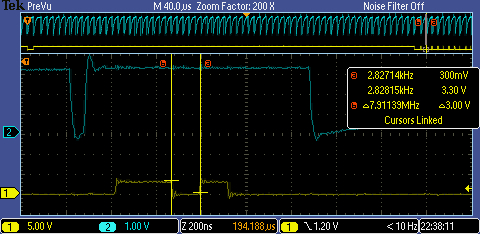
\includegraphics[width=\textwidth]{./img/TEK00001}
    \caption{A data read frame}
    \label{fig:data-frame-0}
  \end{subfigure}
  \begin{subfigure}[b]{0.45\textwidth}
    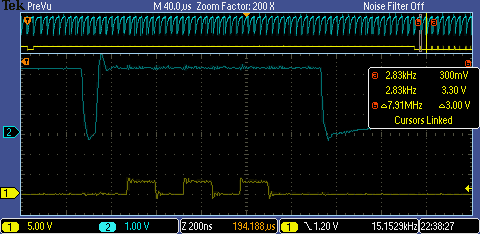
\includegraphics[width=\textwidth]{./img/TEK00002}
    \caption{Another data read frame}
    \label{fig:data-frame-1}
  \end{subfigure}
  \caption{Two SPI packets}
  \label{fig:data-frames}
\end{figure}

\section{Analysis and Discussion}
\begin{enumerate}
\item
  \begin{Ex}
    Does your implementation have external fragmentation? Explain with
    a one sentence answer.
    \begin{solution} \hbr
      no idea
      \todo
    \end{solution}
  \end{Ex}
\item
  \begin{Ex}
    If your disk has ten files, and the number of bytes in each file
    is a random number, what is the expected amount of wasted storage
    due to internal fragmentation? Explain with a one sentence answer.
    \begin{solution} \hbr
      no idea
      \todo
    \end{solution}
  \end{Ex}
\item
  \begin{Ex}
    Assume you replaced the flash memory in the SD card with a high
    speed battery-backed RAM and kept all other hardware/software the
    same. What read/write bandwidth could you expect to achieve?
    Explain with a one sentence answer.
    \begin{solution} \hbr
    In this case, we would be limited by the SPI bandwidth since RAM
    is much faster than SPI. Determine what the spi write
    bandwidth is. Need oscilloscope.
    \todo
    \end{solution}
  \end{Ex}
\item
  \begin{Ex}
    How many files can you store on your disk? Briefly explain how you
    could increase this number (do not do it, just explain how it
    could have been done).
    \begin{solution} \hbr
      no idea
      \todo
    \end{solution}
  \end{Ex}
\item
  \begin{Ex}
    Does your system allow for two threads to simultaneously stream
    debugging data onto one file? If yes, briefly explain how you
    handled the thread synchronization. If not, explain in detail how
    it could have been done. Do not do it, just give 4 or 5 sentences
    and some C code explaining how to handle the synchronization.
    \begin{solution} \hbr
    No. The first thread would have to take a semaphore before a write
    occurs and release it after the write goes through. The second
    thread would have to wait for the semaphore to be released before
    writing the data.
    \end{solution}
  \end{Ex}
\end{enumerate}

\newpage
\section{Code}
\lstinputlisting[language=C,label=lst:lab5,caption=\texttt{lab5.c}]{@doc-staging-area@/lab5.c}
\lstinputlisting[language=C,label=lst:ff-h,caption=\texttt{ff.h}]{@doc-staging-area@/ff.h}
%% \lstinputlisting[language=C,label=lst:ff-c,caption=\texttt{ff.c}]{@doc-staging-area@/ff.c}
\lstinputlisting[language=C,label=lst:shell-h,caption=\texttt{shell.h}]{@doc-staging-area@/shell.h}
\lstinputlisting[language=C,label=lst:shell-c,caption=\texttt{shell.c}]{@doc-staging-area@/shell.c}
\lstinputlisting[language=C,label=lst:system-h,caption=\texttt{system.h}]{@doc-staging-area@/system.h}
\lstinputlisting[language=C,label=lst:system-c,caption=\texttt{system.c}]{@doc-staging-area@/system.c}

\end{document}
